\section{Ziel}
Im folgenden Versuch soll die Charakteristik und Totzeit eines Geiger-Müller-Zählrohrs untersucht werden, welches eingesetzt wird um Strahlung zu detektieren.


\section{Theorie}
\label{sec:Theorie}

\subsection{Aufbau und Funktionsweise des Geiger-Müller-Zählrohrs}
Das Geiger-Müller-Zählrohr besteht aus einem Kathodenzylinder mit einem Durchmesser $d_\textrm{K}=2r_\textrm{K}$. Das Innere des Zylinders ist mit einem Gasgemisch bestehend aus $\SI{100}{\milli\bar}$ Argon und $\SI{10}{\milli\bar}$ Ethyalkohol gefüllt. Außerdem verläuft  parallel zum Rand des Zylinders ein Anodendraht mit dem Radius $2r_\textrm{a}$ .
Eine Seite des Zylinders ist fest verschlossen, die andere Seite ist nur durch eine Mylar-Folie abgedeckt, diese besteht aus einem Material mit niedriger Massenbelegung, sodass $\alpha$-Strahlen sie durchdringen können. Durch den Unterdruck im Zylinder wird die dünne Folie nach innen gewölbt. Der zuvor beschriebene Aufbau ist in Abbildung $\ref{fig:GMZ}$ graphisch dargestellt.
\begin{figure}[H]
  \centering
  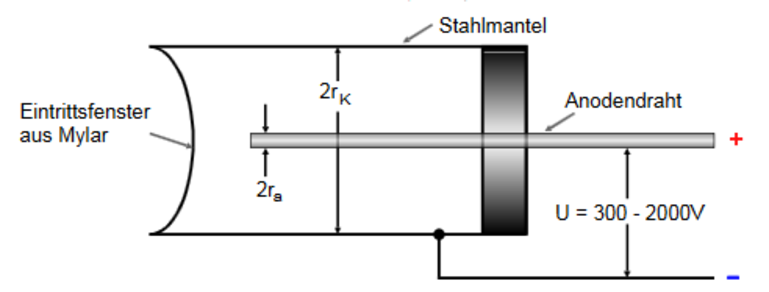
\includegraphics{ressources/G_M_Z.pdf}
  \caption{Aufbau des Geiger-Müller-Zählrohrs, \cite{skript}.}
  \label{fig:GMZ}
\end{figure}

Wird eine Spannung zwischen Anodendraht und Kathodenzylinder angelegt, baut sich ein radialsymmetrischen Feld auf. Die Feldstärke $E(r)$ wird bestimmt durch
\begin{align}
  E(r)= \frac{U}{r \ln{(\frac{r_\textrm{K}}{r_\textrm{a}})}} \;.
  \label{eq:Feldstärke}
\end{align}
Somit wird die Feldstärke $E(r)$ in der Nähe des  Drahtes  maximal.
\subsection{Funktionsweise}
Wie in Abbildung $\ref{fig:Char}$ zu sehen, sind die Abläufe im Zählrohr abhängig von der angelegten Spannung.

\begin{figure}[H]
  \centering
  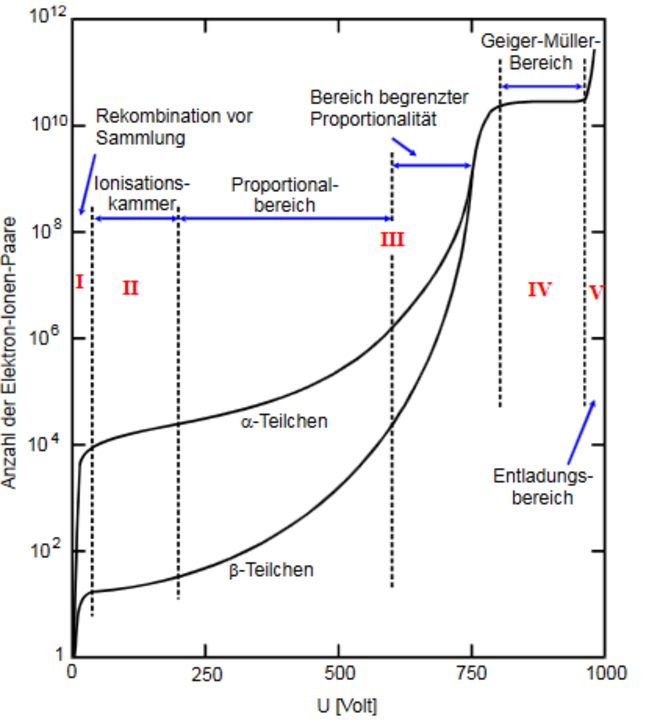
\includegraphics{ressources/charakteristik.pdf}
  \caption{Charakteristik des Geiger-Müller-Zählrohrs samt den im Text beschriebenen Bereichen, \cite{skript}.}
  \label{fig:Char}
\end{figure}

Bei einer niedrigen Spannung erreichen nicht alle einfallenden Teilchen den Anodendraht, da viele Elektronen sich wieder mit einem positiven Ion verbinden und somit zu einem neutral Atom werden.\\
In Bereich 2, ist die Spannung soweit erhöht worden, das eine Rekombination wie in Bereich 1 nicht mehr möglich ist. Somit erreichen alle einfallende Teilchen den Anodendraht und es fließt ein Strom. Dieser Ionisationsstrom ist proportional zur Energie und Intensität der Strahlung. Dabei ist der Strom so gering, dass die sogenannte Ionisationskammer nur bei Quellen mit einer hohen Strahlungsintensität eingesetzt wird.\\
Im nächsten Bereich gewinnen die Elektronen durch die Zusammenstöße mit den Argon-Atomen aufgrund der hohen Feldstärke so viel Energie, dass sie ionisieren. Die durch die Stoßionisation  frei gewordenen Elektronen ionisieren ebenfalls. Der Effekt das sich die Zahl der Elektronen schlagartig vervielfacht nennt man Townsend-Lawine. Der Bereich 3 wird als Proportionalzählrohr bezeichnet, da Aufgrund der proportionalität der einfallenden Teilchen zu der Ladung $Q$, die Energie und die Strahlung gemessen werden kann. \\
Im Bereich 4, wo das Geiger-Müller-Zählrohr agiert, ist die Spannung so hoch, dass die Ladung $Q$ unabhängig von der Primärionisation ist. Desweiteren entstehen durch die Lawinen aus Elektronen UV-Photonen, da Photonen nicht geladen sind, breiten diese sich auch senkrecht zum elektrischen Feld aus. Somit entstehen Townsend-Lawinen im ganzen Rohr. Dadurch ist die Ladung $Q$ am Anodendraht abhängig von dem Volumen des Zylinders. In diesem Spannungsbereich kann nur die Intensität der einfallenden Strahlung gemessen werden.\\
Im letzten Bereich entsteht eine selbständige Gasentlandung, die zu hohen Stromdichten führt und das Zählrohr zerstört.

\subsection{Tot- und Erholungszeit}
Die durch Ionisation entstandenen positiven Ionen sind massereicher als die entstandenen Elektronen, aus diesem Grund halten sich die Ionen länger zwischen Anode und Kathode auf als die Elektronen. Es entsteht ein sogenannter "Ionenschlau". Durch diesen "Ionenschlau" wird die Feldstärke soweit abgeschwächt, das es zu keinen Stoßionisatonen mehr kommen kann. Somit wird ein einfallendes Teilchen in diesem Zeitraum, der Totzeit $T$, nicht detektiert. Registriert das Zählrohr $N_\textrm{r}$ Impulse pro Zeiteinheit, ist das Zählrohr für ein kleines Zeitintervall $TN_\textrm{r}$ nicht funktionsbereit und daher nur für  die restliche Zeit messbereit. Somit ergibt sich die wahre Zählrate $N_\textrm{w}$ durch
\begin{align}
  N_\textrm{w}= \frac{N_\textrm{t}}{1-TN_\textrm{r}}\;.
  \label{eq:N}
\end{align}

Als Erholungszeit $T_\textrm{E}$
wird der Zeitraum bezeichnet indem der Ionisationsschlauch langsam neutralisiert wird. Dadurch ist die Lawinenbildung der Elektronen wieder möglich. Die Erholungszeit $T_\textrm{E}$ ist beendet, wenn die Ladungsimpulse $Q$ ihre ursprüngliche Höhe wieder erreicht haben. Die beiden beschriebenen Zeitabschnitte sind in Abbildung $\ref{fig:Char2}$ dargestellt.

\begin{figure}[H]
  \centering
  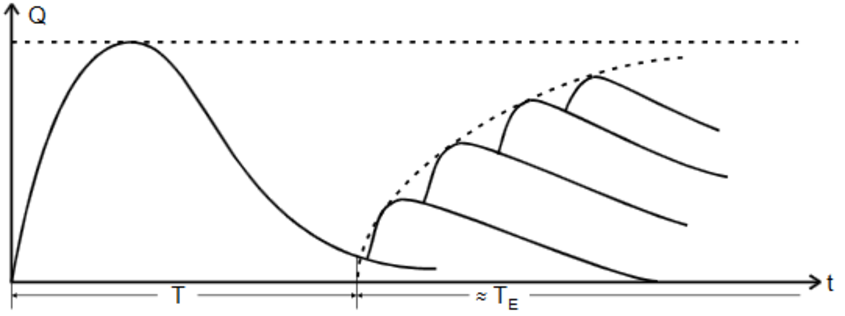
\includegraphics{ressources/Totzeit.pdf}
  \caption{Tot- und Erholungszeit, dargestellt im Ladungs-Zeit-Diagramm, \cite{skript}.}
  \label{fig:Char2}
\end{figure}

\subsection{Nachentladung}
Bei der Neutralisation der Ionen wird so viel Energie frei, dass Elektronen aus der Metalloberfläche ausgelöst werden.  Die frei gewordenen Elektronen werden als "Sekundärelektronen" bezeichnet, da sie das Potential durchlaufen und Zählrohrentladungen erneut verursachen. Aus diesem Grund entstehen aus einem einfallenden Teilchen mehrere Ausgangsimpulse. Da dieses Verhalten unerwünscht ist, wird neben Argon auch Ethyalkohol in den Zylinder gegeben. Die Argon-Ionen stoßen mit den Alkoholmolekülen, daraufhin werden die  Alkoholmoleküle ionisiert und von der Kathode angezogen. An der Kathode angekommen werden sie neutralisiert. Bei diesem Vorgang entstehen jedoch keine weiteren Elektronen. Die entstandene Energie lässt die Alkoholmoleküle schwingen, wodurch die Energie in Wärme umgewandelt wird. Somit werden mehrere Ausgangsimpulse bei nur einem einfallenden Teilchen vermieden.
\subsection{Charakteristik des Zählrohrs}
\label{sec:charakteristik}
Im Geiger-Müller-Bereich bei einer Spannung $U_\textrm{E}$ setzt der Auslösebreich ein. In Abbildung $\ref{fig:Plateau}$ ist zu sehen, wie nach dem Auflösebreich das sogenannte Plateau folgt.  Das Plateau ist ein linearer Abschnitt des Kurvenverlaufs. Je niedriger die Steigung dieser Gerade ist, desto qualitativ hochwertiger ist das Zählrohr. Im Idealfall ist die Plateausteigung null, jedoch werden immer ein paar Nachentladungen entstehen, weshalb im Experiment immer eine Steigung festzustellen ist. Nach dem Plateau folgt der Bereich der Dauerentladung, wo durch hohe Stromdichten das Zählrohr zerstört werden kann.


\begin{figure}[H]
  \centering
  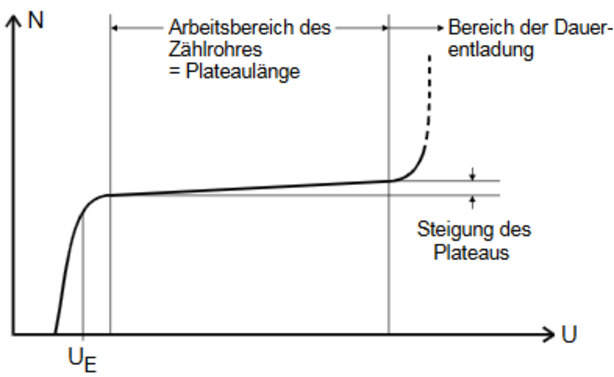
\includegraphics{ressources/Plateau.pdf}
  \caption{Zählrohrcharakteristik im Bereich 4, \cite{skript}.}
  \label{fig:Plateau}
\end{figure}


% 2x2 Plot
% \begin{figure*}
%     \centering
%     \begin{subfigure}[b]{0.475\textwidth}
%         \centering
%         \includegraphics[width=\textwidth]{Abbildungen/Schaltung1.pdf}
%         \caption[]%
%         {{\small Schaltung 1.}}
%         \label{fig:Schaltung1}
%     \end{subfigure}
%     \hfill
%     \begin{subfigure}[b]{0.475\textwidth}
%         \centering
%         \includegraphics[width=\textwidth]{Abbildungen/Schaltung2.pdf}
%         \caption[]%
%         {{\small Schaltung 2.}}
%         \label{fig:Schaltung2}
%     \end{subfigure}
%     \vskip\baselineskip
%     \begin{subfigure}[b]{0.475\textwidth}
%         \centering
%         \includegraphics[width=\textwidth]{Abbildungen/Schaltung4.pdf}    % Zahlen vertauscht ... -.-
%         \caption[]%
%         {{\small Schaltung 3.}}
%         \label{fig:Schaltung3}
%     \end{subfigure}
%     \quad
%     \begin{subfigure}[b]{0.475\textwidth}
%         \centering
%         \includegraphics[width=\textwidth]{Abbildungen/Schaltung3.pdf}
%         \caption[]%
%         {{\small Schaltung 4.}}
%         \label{fig:Schaltung4}
%     \end{subfigure}
%     \caption[]
%     {Ersatzschaltbilder der verschiedenen Teilaufgaben.}
%     \label{fig:Schaltungen}
% \end{figure*}
